\documentclass{beamer}

%
% Common preamble for all three parts.
%

\usetheme[block=fill]{metropolis}
\setbeamercolor{frametitle}{use=normal text, parent=normal text}

\usepackage{arevmath}
\SetSymbolFont{largesymbols}{normal}{OMX}{iwona}{m}{n}
\usepackage{fontspec}
\setmainfont{PT Sans}
\setsansfont{PT Sans}
\setmonofont{PT Mono}[Scale=0.87]
\usepackage[english,russian]{babel}
\usepackage{amsmath}
\usepackage{color}
\usepackage{minted}
\usepackage{hyperref}
\usepackage{multicol}
\usepackage{tabularx}
\usepackage{tikz}
\usepackage{tcolorbox}

% For slide 28 (Tikz examples)
\usetikzlibrary{mindmap,trees}
\usetikzlibrary{backgrounds,shapes,arrows,positioning,calc,snakes,fit}
\usepgflibrary{decorations.markings}

\hypersetup{unicode=true}

\tcbuselibrary{skins}
\tcbuselibrary{listings}
\tcbuselibrary{minted}
\tcbset{colframe=mDarkTeal, colback=white!90!mDarkTeal,% Taken from the Metropolis theme
        left=0.8em,right=0.8em}
\newtcolorbox{tblock}[1]{boxsep=1mm,sidebyside=false,bicolor=false,colback=white,title={#1}}
\newtcolorbox{printout}{boxsep=0mm,sidebyside=false,bicolor=false,colback=white}
\def\linkbox#1{\tcbox[on line,boxsep=0mm,left=2pt,right=2pt,top=2pt,bottom=2pt,
                      colback=mDarkTeal,coltext=white]{#1}}
\def\ovllink#1{\tcbox[on line,boxsep=0mm,left=2pt,right=2pt,top=2pt,bottom=2pt,
                      colback=green!30!black,colframe=green!30!black,coltext=white]{#1}}
\newtcblisting{code}{boxsep=0mm,listing only,minted language=latex}
\newtcblisting{bibtexcode}{boxsep=0mm,listing only,minted language=bibtex}
\newtcblisting{exampletwoup}{fontupper=\small,fontlower=\small,
                             boxsep=0mm,listing side text,minted language=latex,
                             bicolor,colbacklower=white,
                             righthand ratio=0.42}
\newtcblisting{exampletwouptiny}{fontupper=\footnotesize,fontlower=\footnotesize,
                                 boxsep=0mm,listing side text,minted language=latex,
                                 minted options={fontsize=\footnotesize},
                                 bicolor,colbacklower=white,
                                 righthand ratio=0.42}
\newtcblisting{exampletwouppaused}{fontupper=\footnotesize,fontlower=\footnotesize,
                             boxsep=0mm,listing side text,minted language=latex,
                             minted options={fontsize=\footnotesize},
                             bicolor,colbacklower=white,
                             righthand ratio=0.42,after lower=\onslide<1->}
\newtcbinputlisting{\inputcode}[2][]{%
listing file={#2},boxsep=0mm,listing only,minted language=latex,#1}
\newtcbinputlisting{\inputbibtexcode}[2][]{%
listing file={#2},boxsep=0mm,listing only,minted language=bibtex,#1}

% only inline todonotes work
\usepackage{xkeyval}
\usepackage[textsize=small]{todonotes}
\presetkeys{todonotes}{inline}{}

\usetikzlibrary{shapes,arrows,positioning,shadows}

% no nav buttons
\usenavigationsymbolstemplate{}

\newcommand{\bftt}[1]{\textbf{\texttt{#1}}}
%\newcommand{\comment}[1]{{\color[HTML]{008080}\textit{\textbf{\texttt{#1}}}}}
\newcommand{\cmd}[1]{{\color[HTML]{008000}\bftt{#1}}}
\newcommand{\bs}{\char`\\}
\newcommand{\cmdbs}[1]{\cmd{\bs#1}}
\newcommand{\lcb}{\char '173}
\newcommand{\rcb}{\char '175}
\newcommand{\cmdbegin}[1]{\cmdbs{begin\lcb}\bftt{#1}\cmd{\rcb}}
\newcommand{\cmdend}[1]{\cmdbs{end\lcb}\bftt{#1}\cmd{\rcb}}

\newcommand{\wllogo}{\textbf{Overleaf}}

% this is where the example source files are loaded from
% do not include a trailing slash
\newcommand{\fileuri}{https://raw.github.com/sgolovan/latex-course/master/ru}

\newcommand{\wlserver}{https://www.overleaf.com}
\newcommand{\wlnewdoc}[1]{\wlserver/docs?snip\_uri=\fileuri/#1\&splash=none}

\def\tikzname{Ti\emph{k}Z}

% from http://tex.stackexchange.com/questions/5226/keyboard-font-for-latex
\newcommand*\keystroke[1]{%
  \tikz[baseline=(key.base)]
    \node[%
      draw,
      fill=white,
      drop shadow={shadow xshift=0.25ex,shadow yshift=-0.25ex,fill=black,opacity=0.75},
      rectangle,
      rounded corners=2pt,
      inner sep=1pt,
      line width=0.5pt,
      font=\scriptsize\ttfamily
    ](key) {#1\strut}
  ;
}
\newcommand{\keystrokebftt}[1]{\keystroke{\bftt{#1}}}

% stolen from minted.dtx
\newenvironment{exampletwouptinynoframe}
  {\VerbatimEnvironment
   \begin{VerbatimOut}{example.out}}
  {\end{VerbatimOut}
   \setlength{\parindent}{0pt}
   \begin{tabular}{l|l}
   \begin{minipage}{0.55\linewidth}
     \inputminted[fontsize=\scriptsize,resetmargins]{latex}{example.out}
   \end{minipage} &
   \begin{minipage}{0.35\linewidth}
     \setlength{\parskip}{6pt plus 1pt minus 1pt}%
     \raggedright\scriptsize\input{example.out}
   \end{minipage}
   \end{tabular}}

\title{Интерактивное введение в \LaTeX}
\author{Джон Д. Лис-Миллер\\Перевод на русский язык: Сергей Головань}
%\titlegraphic{%
%\includegraphics[height=36pt]{overleaf}\\[1em]
%\includegraphics[height=24pt]{UoB-logo}
%}


\subtitle{Часть 2: Структурированные документы \& ещё кое что}

\begin{document}

%%%%%%%%%%%%%%%%%%%%%%%%%%%%%%%%%%%%%%%%%%%%%%%%%%%%%%%%%%%%%%%%%%%%%%%%%%%%%%%
%%%%%%%%%%%%%%%%%%%%%%%%%%%%%%%%%%%%%%%%%%%%%%%%%%%%%%%%%%%%%%%%%%%%%%%%%%%%%%%
%%%%%%%%%%%%%%%%%%%%%%%%%%%%%%%%%%%%%%%%%%%%%%%%%%%%%%%%%%%%%%%%%%%%%%%%%%%%%%%
\begin{frame}
\titlepage
\end{frame}

%%%%%%%%%%%%%%%%%%%%%%%%%%%%%%%%%%%%%%%%%%%%%%%%%%%%%%%%%%%%%%%%%%%%%%%%%%%%%%%
%%%%%%%%%%%%%%%%%%%%%%%%%%%%%%%%%%%%%%%%%%%%%%%%%%%%%%%%%%%%%%%%%%%%%%%%%%%%%%%
%%%%%%%%%%%%%%%%%%%%%%%%%%%%%%%%%%%%%%%%%%%%%%%%%%%%%%%%%%%%%%%%%%%%%%%%%%%%%%%
\section{Структурированные документы}

%%%%%%%%%%%%%%%%%%%%%%%%%%%%%%%%%%%%%%%%%%%%%%%%%%%%%%%%%%%%%%%%%%%%%%%%%%%%%%%
%%%%%%%%%%%%%%%%%%%%%%%%%%%%%%%%%%%%%%%%%%%%%%%%%%%%%%%%%%%%%%%%%%%%%%%%%%%%%%%
%%%%%%%%%%%%%%%%%%%%%%%%%%%%%%%%%%%%%%%%%%%%%%%%%%%%%%%%%%%%%%%%%%%%%%%%%%%%%%%
\begin{frame}{Обзор}
\begin{multicols}{2}
\tableofcontents[currentsection]
\end{multicols}
\end{frame}

%%%%%%%%%%%%%%%%%%%%%%%%%%%%%%%%%%%%%%%%%%%%%%%%%%%%%%%%%%%%%%%%%%%%%%%%%%%%%%%
%%%%%%%%%%%%%%%%%%%%%%%%%%%%%%%%%%%%%%%%%%%%%%%%%%%%%%%%%%%%%%%%%%%%%%%%%%%%%%%
%%%%%%%%%%%%%%%%%%%%%%%%%%%%%%%%%%%%%%%%%%%%%%%%%%%%%%%%%%%%%%%%%%%%%%%%%%%%%%%
\begin{frame}{\insertsection}
\begin{itemize}
\item In Part 1, we learned about commands and environments for typesetting text
and mathematics.
\item Now, we'll learn about commands and environments for structuring
documents.
\item You can try out the new commands in Overleaf:
\end{itemize}
\vskip 2em
\begin{center}
\fbox{\href{\wlnewdoc{basics.tex}}{%
Click here to open the example document in \wllogo{}}}
\\[1ex]\scriptsize{}
For best results, please use \href{http://www.google.com/chrome}{Google Chrome} or a recent \href{http://www.mozilla.org/en-US/firefox/new/}{FireFox}.
\end{center}
\vskip 2ex
\begin{itemize}
\item Let's get started!
\end{itemize}
\end{frame}

%%%%%%%%%%%%%%%%%%%%%%%%%%%%%%%%%%%%%%%%%%%%%%%%%%%%%%%%%%%%%%%%%%%%%%%%%%%%%%%
%%%%%%%%%%%%%%%%%%%%%%%%%%%%%%%%%%%%%%%%%%%%%%%%%%%%%%%%%%%%%%%%%%%%%%%%%%%%%%%
%%%%%%%%%%%%%%%%%%%%%%%%%%%%%%%%%%%%%%%%%%%%%%%%%%%%%%%%%%%%%%%%%%%%%%%%%%%%%%%
\subsection{Название и аннотация}
\begin{frame}[fragile]{\insertsubsection}
\vspace{-2ex}
\begin{itemize}{\small
\item Укажите \LaTeX{}'у \cmdbs{title} и \cmdbs{author} в преамбуле.
\item Далее воспользуйтесь \cmdbs{maketitle} в документе, чтобы вывести название.
\item Для печати аннотации применяется окружение \bftt{abstract}.
}\end{itemize}
\vspace{-2ex}
\begin{minipage}{0.55\linewidth}
\inputcode[minted options={fontsize=\footnotesize}]{structure-title.tex}
\end{minipage}~~%
\begin{minipage}{0.45\linewidth}
\includegraphics[width=\textwidth,clip,viewport=0cm 227mm 5cm 297mm]{structure-title.pdf}
\end{minipage}
\end{frame}

%%%%%%%%%%%%%%%%%%%%%%%%%%%%%%%%%%%%%%%%%%%%%%%%%%%%%%%%%%%%%%%%%%%%%%%%%%%%%%%
%%%%%%%%%%%%%%%%%%%%%%%%%%%%%%%%%%%%%%%%%%%%%%%%%%%%%%%%%%%%%%%%%%%%%%%%%%%%%%%
%%%%%%%%%%%%%%%%%%%%%%%%%%%%%%%%%%%%%%%%%%%%%%%%%%%%%%%%%%%%%%%%%%%%%%%%%%%%%%%
\subsection{Разделы}
\begin{frame}{\insertsubsection}
\vspace{-2ex}
\begin{itemize}{\small
\item Просто указывайте \cmdbs{section} или \cmdbs{subsection}.
\item Угадайте, что делают команды \cmdbs{section*} и \cmdbs{subsection*}?
}\end{itemize}
\begin{minipage}{0.55\linewidth}
\inputcode[minted options={fontsize=\footnotesize}]{structure-sections.tex}
\end{minipage}~~%
\begin{minipage}{0.45\linewidth}
\includegraphics[width=\textwidth,clip,viewport=0cm 227mm 5cm 297mm]{structure-sections.pdf}
\end{minipage}
\end{frame}

%%%%%%%%%%%%%%%%%%%%%%%%%%%%%%%%%%%%%%%%%%%%%%%%%%%%%%%%%%%%%%%%%%%%%%%%%%%%%%%
%%%%%%%%%%%%%%%%%%%%%%%%%%%%%%%%%%%%%%%%%%%%%%%%%%%%%%%%%%%%%%%%%%%%%%%%%%%%%%%
%%%%%%%%%%%%%%%%%%%%%%%%%%%%%%%%%%%%%%%%%%%%%%%%%%%%%%%%%%%%%%%%%%%%%%%%%%%%%%%
\subsection{Метки и перекрёстные ссылки}
\begin{frame}[fragile]{\insertsubsection}
\vspace{-2ex}
\begin{itemize}{\small
\item Применяйте \cmdbs{label} и \cmdbs{ref} для автоматических ссылок.
\item Пакет \bftt{amsmath} предоставляет \cmdbs{eqref} для ссылок на уравнения.
}\end{itemize}
\begin{minipage}{0.55\linewidth}
\inputcode[minted options={fontsize=\scriptsize}]{structure-crossref.tex}
\end{minipage}~~%
\begin{minipage}{0.45\linewidth}
\includegraphics[width=\textwidth,clip,viewport=0cm 227mm 5cm 297mm]{structure-crossref.pdf}
\end{minipage}
\end{frame}

%%%%%%%%%%%%%%%%%%%%%%%%%%%%%%%%%%%%%%%%%%%%%%%%%%%%%%%%%%%%%%%%%%%%%%%%%%%%%%%
%%%%%%%%%%%%%%%%%%%%%%%%%%%%%%%%%%%%%%%%%%%%%%%%%%%%%%%%%%%%%%%%%%%%%%%%%%%%%%%
%%%%%%%%%%%%%%%%%%%%%%%%%%%%%%%%%%%%%%%%%%%%%%%%%%%%%%%%%%%%%%%%%%%%%%%%%%%%%%%
\subsection{Упражнение}
\begin{frame}[fragile]{Упражнение на структурные документы}

\begin{tblock}{Наберите этот короткий документ в \LaTeX:\footnotemark}
\begin{printout}
\href{\fileuri/structure-exercise-solution.pdf}{%
Click to open the paper}
\end{printout}
Make your paper look like this one. Use \cmdbs{ref} and \cmdbs{eqref} to avoid
explicitly writing section and equation numbers into the text.
\end{tblock}
\footnotetext{From \url{http://pdos.csail.mit.edu/scigen/}, a random
paper generator.}
\vskip 2ex
\begin{printout}
\href{\wlnewdoc{structure-exercise.tex}}{%
Click to open this exercise in \wllogo{}}
\end{printout}

\begin{itemize}
\item Once you've tried,
\ovllink{\href{\wlnewdoc{structure-exercise-solution.tex}}{%
click here to see my solution}}.
\end{itemize}
\end{frame}

%%%%%%%%%%%%%%%%%%%%%%%%%%%%%%%%%%%%%%%%%%%%%%%%%%%%%%%%%%%%%%%%%%%%%%%%%%%%%%%
%%%%%%%%%%%%%%%%%%%%%%%%%%%%%%%%%%%%%%%%%%%%%%%%%%%%%%%%%%%%%%%%%%%%%%%%%%%%%%%
%%%%%%%%%%%%%%%%%%%%%%%%%%%%%%%%%%%%%%%%%%%%%%%%%%%%%%%%%%%%%%%%%%%%%%%%%%%%%%%
\section{Figures and Tables}

%%%%%%%%%%%%%%%%%%%%%%%%%%%%%%%%%%%%%%%%%%%%%%%%%%%%%%%%%%%%%%%%%%%%%%%%%%%%%%%
%%%%%%%%%%%%%%%%%%%%%%%%%%%%%%%%%%%%%%%%%%%%%%%%%%%%%%%%%%%%%%%%%%%%%%%%%%%%%%%
%%%%%%%%%%%%%%%%%%%%%%%%%%%%%%%%%%%%%%%%%%%%%%%%%%%%%%%%%%%%%%%%%%%%%%%%%%%%%%%
\begin{frame}{Outline}
\begin{multicols}{2}
\tableofcontents[currentsection]
\end{multicols}
\end{frame}

%%%%%%%%%%%%%%%%%%%%%%%%%%%%%%%%%%%%%%%%%%%%%%%%%%%%%%%%%%%%%%%%%%%%%%%%%%%%%%%
%%%%%%%%%%%%%%%%%%%%%%%%%%%%%%%%%%%%%%%%%%%%%%%%%%%%%%%%%%%%%%%%%%%%%%%%%%%%%%%
%%%%%%%%%%%%%%%%%%%%%%%%%%%%%%%%%%%%%%%%%%%%%%%%%%%%%%%%%%%%%%%%%%%%%%%%%%%%%%%
\subsection{Graphics}
\begin{frame}[fragile]{\insertsubsection}
\begin{itemize}
\item Requires the \bftt{graphicx} package, which provides the
\cmdbs{includegraphics} command.
\item Supported graphics formats include JPEG, PNG and PDF (usually).
\end{itemize}
\begin{exampletwouptiny}
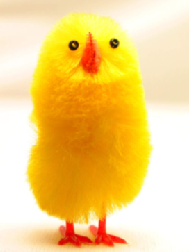
\includegraphics[
  width=0.5\textwidth]{big_chick}

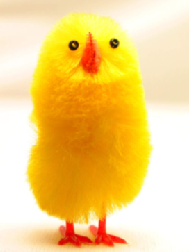
\includegraphics[
  width=0.3\textwidth,
  angle=270]{big_chick}
\end{exampletwouptiny}

\tiny{Image from \url{http://www.andy-roberts.net/writing/latex/importing_images}}
\end{frame}

%%%%%%%%%%%%%%%%%%%%%%%%%%%%%%%%%%%%%%%%%%%%%%%%%%%%%%%%%%%%%%%%%%%%%%%%%%%%%%%
%%%%%%%%%%%%%%%%%%%%%%%%%%%%%%%%%%%%%%%%%%%%%%%%%%%%%%%%%%%%%%%%%%%%%%%%%%%%%%%
%%%%%%%%%%%%%%%%%%%%%%%%%%%%%%%%%%%%%%%%%%%%%%%%%%%%%%%%%%%%%%%%%%%%%%%%%%%%%%%
\begin{frame}[fragile]{Interlude: Optional Arguments}
\begin{itemize}
\item We use square brackets \keystrokebftt{[} \keystrokebftt{]} for optional
arguments, instead of braces \keystrokebftt{\{} \keystrokebftt{\}}.
\item \cmdbs{includegraphics} accepts optional arguments that allow you to transform the
image when it is included. For example, \bftt{width=0.3\cmdbs{textwidth}} makes
the image take up 30\% of the width of the surrounding text (\cmdbs{textwidth}).
\item \cmdbs{documentclass} accepts optional arguments, too. Example:
\mint{latex}|\documentclass[12pt,twocolumn]{article}|
\vskip 3ex
makes the text bigger (12pt) and puts it into two columns.
\item Where do you find out about these? See the slides at the end of this
presentation for links to more information.
\end{itemize}
\end{frame}

%%%%%%%%%%%%%%%%%%%%%%%%%%%%%%%%%%%%%%%%%%%%%%%%%%%%%%%%%%%%%%%%%%%%%%%%%%%%%%%
%%%%%%%%%%%%%%%%%%%%%%%%%%%%%%%%%%%%%%%%%%%%%%%%%%%%%%%%%%%%%%%%%%%%%%%%%%%%%%%
%%%%%%%%%%%%%%%%%%%%%%%%%%%%%%%%%%%%%%%%%%%%%%%%%%%%%%%%%%%%%%%%%%%%%%%%%%%%%%%
\subsection[fragile]{Плавающие объекты}

\begin{frame}{\insertsubsection}
\vspace{-2ex}
\begin{itemize}
\item Позвольте \LaTeX{} решить, куда поставить рисунок (он может <<плавать>>).
\item Также можно снабдить рисунок номером и подписью, на которые потом можно
  ссылаться с помощью \cmdbs{ref}.
\end{itemize}
\vspace{-6ex}
\begin{minipage}[t]{0.55\linewidth}
\inputcode[minted options={fontsize=\scriptsize}]{media-graphics.tex}
\end{minipage}~~%
\begin{minipage}[t]{0.45\linewidth}
\includegraphics[width=\textwidth,clip,viewport=0cm 227mm 5cm 297mm]{media-graphics.pdf}
\end{minipage}
\end{frame}

%%%%%%%%%%%%%%%%%%%%%%%%%%%%%%%%%%%%%%%%%%%%%%%%%%%%%%%%%%%%%%%%%%%%%%%%%%%%%%%
%%%%%%%%%%%%%%%%%%%%%%%%%%%%%%%%%%%%%%%%%%%%%%%%%%%%%%%%%%%%%%%%%%%%%%%%%%%%%%%
%%%%%%%%%%%%%%%%%%%%%%%%%%%%%%%%%%%%%%%%%%%%%%%%%%%%%%%%%%%%%%%%%%%%%%%%%%%%%%%
\subsection{Таблицы}

\begin{frame}[fragile]{\insertsubsection}
\vspace{-3ex}
\begin{itemize}
\item Чтобы привыкнуть к таблицам в \LaTeX{}, нужно время.
\item Можно воспользоваться окружением \bftt{tabular}.
\item Аргумент задаёт выравнивание колонок --- \textbf{l}eft, \textbf{r}ight, \textbf{r}ight.
\begin{exampletwouptiny}
\begin{tabular}{lrr}
Прод.  & \# & Цена \$ \\
Гаджет & 1  & 199.99  \\
Виджет & 2  & 399.99  \\
Кабель & 3  & 19.99   \\
\end{tabular}
\end{exampletwouptiny}
\vspace{-1ex}
\item В нём также задаются вертикальные линии; команда \cmdbs{hline} проводит горизонтальную линию.
\begin{exampletwouptiny}
\begin{tabular}{|l|r|r|} \hline
Прод.  & \# & Цена \$ \\\hline
Виджет & 1  & 199.99  \\
Гаджет & 2  & 399.99  \\
Кабель & 3  & 19.99   \\\hline
\end{tabular}
\end{exampletwouptiny}
\item Use an ampersand \keystrokebftt{\&} to separate columns and a double backslash \keystrokebftt{\bs}\keystrokebftt{\bs} to start a new row (like in the \bftt{align*} environment that we saw in part 1).
\end{itemize}
\end{frame}

%%%%%%%%%%%%%%%%%%%%%%%%%%%%%%%%%%%%%%%%%%%%%%%%%%%%%%%%%%%%%%%%%%%%%%%%%%%%%%%
%%%%%%%%%%%%%%%%%%%%%%%%%%%%%%%%%%%%%%%%%%%%%%%%%%%%%%%%%%%%%%%%%%%%%%%%%%%%%%%
%%%%%%%%%%%%%%%%%%%%%%%%%%%%%%%%%%%%%%%%%%%%%%%%%%%%%%%%%%%%%%%%%%%%%%%%%%%%%%%
\addtocontents{toc}{\newpage}
\section{Библиография}

%%%%%%%%%%%%%%%%%%%%%%%%%%%%%%%%%%%%%%%%%%%%%%%%%%%%%%%%%%%%%%%%%%%%%%%%%%%%%%%
%%%%%%%%%%%%%%%%%%%%%%%%%%%%%%%%%%%%%%%%%%%%%%%%%%%%%%%%%%%%%%%%%%%%%%%%%%%%%%%
%%%%%%%%%%%%%%%%%%%%%%%%%%%%%%%%%%%%%%%%%%%%%%%%%%%%%%%%%%%%%%%%%%%%%%%%%%%%%%%
\begin{frame}{Обзор}
\begin{multicols}{2}
\tableofcontents[currentsection]
\end{multicols}
\end{frame}

%%%%%%%%%%%%%%%%%%%%%%%%%%%%%%%%%%%%%%%%%%%%%%%%%%%%%%%%%%%%%%%%%%%%%%%%%%%%%%%
%%%%%%%%%%%%%%%%%%%%%%%%%%%%%%%%%%%%%%%%%%%%%%%%%%%%%%%%%%%%%%%%%%%%%%%%%%%%%%%
%%%%%%%%%%%%%%%%%%%%%%%%%%%%%%%%%%%%%%%%%%%%%%%%%%%%%%%%%%%%%%%%%%%%%%%%%%%%%%%
\subsection{Biblatex}
\begin{frame}[fragile]{\insertsubsection{} 1}
\vspace{-2ex}
\begin{itemize}
\item Сохраните ваши ссылки в \bftt{.bib} файле формата `bibtex':
\inputbibtexcode[minted options={fontsize=\scriptsize}]{bib-example.bib}
\item Большинство менеджеров ссылок могут экспортировать в формат bibtex.
\end{itemize}
\end{frame}

%%%%%%%%%%%%%%%%%%%%%%%%%%%%%%%%%%%%%%%%%%%%%%%%%%%%%%%%%%%%%%%%%%%%%%%%%%%%%%%
%%%%%%%%%%%%%%%%%%%%%%%%%%%%%%%%%%%%%%%%%%%%%%%%%%%%%%%%%%%%%%%%%%%%%%%%%%%%%%%
%%%%%%%%%%%%%%%%%%%%%%%%%%%%%%%%%%%%%%%%%%%%%%%%%%%%%%%%%%%%%%%%%%%%%%%%%%%%%%%
\begin{frame}[fragile]{\insertsubsection{} 2}
\begin{itemize}
\item Каждый элемент в \bftt{.bib} файле включает \emph{ключ}, с помощью которого
на него можно ссылаться в документе. Например, \bftt{semenov2003paradox} это
ключ для этой статьи:
\begin{bibtexcode}
@article{semenov2003paradox,
  author = {Семёнов, Владимир},
}
\end{bibtexcode}
\item Хорошие ключи получаются из комбинаций имени автора, года и названия.
\item \LaTeX{} с помощью пакета \bftt{biblatex} автоматически отформатирует
цитаты в тексте и сгенерирует список литературы; он поддерживает большинство
стандартных стилей, но вы всегда можете разработать свой собственный.
\end{itemize}
\end{frame}

%%%%%%%%%%%%%%%%%%%%%%%%%%%%%%%%%%%%%%%%%%%%%%%%%%%%%%%%%%%%%%%%%%%%%%%%%%%%%%%
%%%%%%%%%%%%%%%%%%%%%%%%%%%%%%%%%%%%%%%%%%%%%%%%%%%%%%%%%%%%%%%%%%%%%%%%%%%%%%%
%%%%%%%%%%%%%%%%%%%%%%%%%%%%%%%%%%%%%%%%%%%%%%%%%%%%%%%%%%%%%%%%%%%%%%%%%%%%%%%
\begin{frame}[fragile]{\insertsubsection{} 3}
\vspace{-3ex}
\small
\begin{itemize}
\item Используйте пакет \bftt{biblatex}\footnote{\scriptsize Многие шаблоны статей используют
\bftt{natbib} вместе с \bftt{bibtex}. Но эта связка не поддерживает русский язык.}
и команды \cmdbs{cite} and \cmdbs{parencite}.
\item Включите файл со ссылками через \cmdbs{addbibresource} и выведите список
литературы через \cmdbs{printbibliography}.
\end{itemize}
\vspace{-2ex}
\begin{minipage}{0.55\linewidth}
\inputcode[minted options={fontsize=\scriptsize}]{bib-example.tex}
\end{minipage}~~%
\begin{minipage}{0.45\linewidth}
\includegraphics[width=\textwidth,clip,viewport=0cm 232mm 5.2cm 297mm]{bib-example.pdf}
\end{minipage}
\end{frame}

%%%%%%%%%%%%%%%%%%%%%%%%%%%%%%%%%%%%%%%%%%%%%%%%%%%%%%%%%%%%%%%%%%%%%%%%%%%%%%%
%%%%%%%%%%%%%%%%%%%%%%%%%%%%%%%%%%%%%%%%%%%%%%%%%%%%%%%%%%%%%%%%%%%%%%%%%%%%%%%
%%%%%%%%%%%%%%%%%%%%%%%%%%%%%%%%%%%%%%%%%%%%%%%%%%%%%%%%%%%%%%%%%%%%%%%%%%%%%%%
\subsection{Exercise}
\begin{frame}[fragile]{Exercise: Putting it All Together}

Add an image and a bibliography to the paper from the previous exercise.

\begin{enumerate}
\item Download these example files to your computer.

\begin{center}
\fbox{\href{\fileuri/big_chick.png?dl=1}{Click to download example image}}

\fbox{\href{\fileuri/bib-exercise.bib?dl=1}{Click to download example bib file}}
\end{center}

\item Upload them to Overleaf (use the project menu).

\end{enumerate}
\end{frame}

%%%%%%%%%%%%%%%%%%%%%%%%%%%%%%%%%%%%%%%%%%%%%%%%%%%%%%%%%%%%%%%%%%%%%%%%%%%%%%%
%%%%%%%%%%%%%%%%%%%%%%%%%%%%%%%%%%%%%%%%%%%%%%%%%%%%%%%%%%%%%%%%%%%%%%%%%%%%%%%
%%%%%%%%%%%%%%%%%%%%%%%%%%%%%%%%%%%%%%%%%%%%%%%%%%%%%%%%%%%%%%%%%%%%%%%%%%%%%%%
\section{What's Next?}

%%%%%%%%%%%%%%%%%%%%%%%%%%%%%%%%%%%%%%%%%%%%%%%%%%%%%%%%%%%%%%%%%%%%%%%%%%%%%%%
%%%%%%%%%%%%%%%%%%%%%%%%%%%%%%%%%%%%%%%%%%%%%%%%%%%%%%%%%%%%%%%%%%%%%%%%%%%%%%%
%%%%%%%%%%%%%%%%%%%%%%%%%%%%%%%%%%%%%%%%%%%%%%%%%%%%%%%%%%%%%%%%%%%%%%%%%%%%%%%
\begin{frame}{Outline}
\begin{multicols}{2}
\tableofcontents[currentsection]
\end{multicols}
\end{frame}

%%%%%%%%%%%%%%%%%%%%%%%%%%%%%%%%%%%%%%%%%%%%%%%%%%%%%%%%%%%%%%%%%%%%%%%%%%%%%%%
%%%%%%%%%%%%%%%%%%%%%%%%%%%%%%%%%%%%%%%%%%%%%%%%%%%%%%%%%%%%%%%%%%%%%%%%%%%%%%%
%%%%%%%%%%%%%%%%%%%%%%%%%%%%%%%%%%%%%%%%%%%%%%%%%%%%%%%%%%%%%%%%%%%%%%%%%%%%%%%
\subsection{More Neat Things}
\begin{frame}[fragile]{\insertsubsection}
\begin{itemize}
\item Add the \cmdbs{tableofcontents} command to generate a table of contents
from the \cmdbs{section} commands.

\item Change the \cmdbs{documentclass} to
\mint{latex}!\documentclass{scrartcl}!
or
\mint{latex}!\documentclass[12pt]{IEEEtran}!

\item Define your own command for a complicated equation:
\begin{exampletwouptiny}
\newcommand{\rperf}{%
  \rho_{\text{perf}}}
$$
\rperf = {\bf c}'{\bf X} + \varepsilon
$$
\end{exampletwouptiny}
\end{itemize}
\end{frame}

%%%%%%%%%%%%%%%%%%%%%%%%%%%%%%%%%%%%%%%%%%%%%%%%%%%%%%%%%%%%%%%%%%%%%%%%%%%%%%%
%%%%%%%%%%%%%%%%%%%%%%%%%%%%%%%%%%%%%%%%%%%%%%%%%%%%%%%%%%%%%%%%%%%%%%%%%%%%%%%
%%%%%%%%%%%%%%%%%%%%%%%%%%%%%%%%%%%%%%%%%%%%%%%%%%%%%%%%%%%%%%%%%%%%%%%%%%%%%%%
\subsection{More Neat Packages}
\begin{frame}{\insertsubsection}
\begin{itemize}
\item \bftt{beamer}: for presentations (like this one!)
\item \bftt{todonotes}: comments and TODO management
\item \bftt{tikz}: make amazing graphics
\item \bftt{pgfplots}: create graphs in \LaTeX
\item \bftt{listings}: source code printer for \LaTeX
\item \bftt{spreadtab}: create spreadsheets in \LaTeX
\item \bftt{gchords}, \bftt{guitar}: guitar chords and tabulature
\item \bftt{cwpuzzle}: crossword puzzles
\end{itemize}
See \url{https://www.overleaf.com/latex/examples} and \url{http://texample.net}
for examples of (most of) these packages.
\end{frame}

%%%%%%%%%%%%%%%%%%%%%%%%%%%%%%%%%%%%%%%%%%%%%%%%%%%%%%%%%%%%%%%%%%%%%%%%%%%%%%%
%%%%%%%%%%%%%%%%%%%%%%%%%%%%%%%%%%%%%%%%%%%%%%%%%%%%%%%%%%%%%%%%%%%%%%%%%%%%%%%
%%%%%%%%%%%%%%%%%%%%%%%%%%%%%%%%%%%%%%%%%%%%%%%%%%%%%%%%%%%%%%%%%%%%%%%%%%%%%%%
\subsection{Installing \LaTeX{}}
\begin{frame}{\insertsubsection}
\begin{itemize}
\item To run \LaTeX{} on your own computer, you'll want to use a \LaTeX{}
\emph{distribution}. A distribution includes a \bftt{latex} program
and (typically) several thousand packages.
\begin{itemize}
\item On Windows: \href{http://miktex.org/}{Mik\TeX} or \href{http://tug.org/texlive/}{\TeX Live}
\item On Linux: \href{http://tug.org/texlive/}{\TeX Live}
\item On Mac: \href{http://tug.org/mactex/}{Mac\TeX}
\end{itemize}
\item You'll also want a text editor with \LaTeX{} support. See \url{http://en.wikipedia.org/wiki/Comparison_of_TeX_editors} for a list of (many) options.
\item You'll also have to know more about how \bftt{latex} and its related tools
work --- see the resources on the next slide.
\end{itemize}
\end{frame}

%%%%%%%%%%%%%%%%%%%%%%%%%%%%%%%%%%%%%%%%%%%%%%%%%%%%%%%%%%%%%%%%%%%%%%%%%%%%%%%
%%%%%%%%%%%%%%%%%%%%%%%%%%%%%%%%%%%%%%%%%%%%%%%%%%%%%%%%%%%%%%%%%%%%%%%%%%%%%%%
%%%%%%%%%%%%%%%%%%%%%%%%%%%%%%%%%%%%%%%%%%%%%%%%%%%%%%%%%%%%%%%%%%%%%%%%%%%%%%%
\subsection{Online Resources}
\begin{frame}{\insertsubsection}
\begin{itemize}
\item \href{http://en.wikibooks.org/wiki/LaTeX}{The \LaTeX{} Wikibook} ---
excellent tutorials and reference material.
\item \href{http://tex.stackexchange.com/}{\TeX{} Stack Exchange} --- ask
questions and get excellent answers incredibly quickly
\item \href{http://www.latex-community.org/}{\LaTeX{} Community} --- a large
online forum
\item \href{http://ctan.org/}{Comprehensive \TeX{} Archive Network (CTAN)} ---
over four thousand packages plus documentation
\item Google will usually get you to one of the above.
\end{itemize}
\end{frame}

%%%%%%%%%%%%%%%%%%%%%%%%%%%%%%%%%%%%%%%%%%%%%%%%%%%%%%%%%%%%%%%%%%%%%%%%%%%%%%%
%%%%%%%%%%%%%%%%%%%%%%%%%%%%%%%%%%%%%%%%%%%%%%%%%%%%%%%%%%%%%%%%%%%%%%%%%%%%%%%
%%%%%%%%%%%%%%%%%%%%%%%%%%%%%%%%%%%%%%%%%%%%%%%%%%%%%%%%%%%%%%%%%%%%%%%%%%%%%%%
\begin{frame}
\begin{center}
Thanks, and happy \TeX{}ing!
\end{center}
\end{frame}

\end{document}

% -- latex understands words, sentences and paragraphs

Words are separated by one or more spaces.  Paragraphs are separated by
one or more blank lines.  The output is not affected by adding extra
spaces or extra blank lines to the input file.

Double quotes are typed like this: ``quoted text''.
Single quotes are typed like this: `single-quoted text'.

Emphasized text is typed like this: \emph{this is emphasized}.
Bold       text is typed like this: \textbf{this is bold}.

-- Adding structure to your document

\section{Hello}

\subsection{World}

\subsection{Foo}

\subsubsection*{Stuff} % star form

\subsubsection*{Results}

-- Labels and cross-references

\label{sec:intro}
\label{sec:method}
\ref{sec:method}

--> maybe introduce the prettyref package here.

-- Mathematics

Inline mathematics: $x + y < 7$.

'Displayed' mathematics:
\begin{equation}
\end{equation}

\begin{equation*}
\end{equation*}

\begin{align}
\end{align}

-- Figures

- Need the graphicx package.

- here we can start introducing options

\includegraphics[width=\textwidth]{}

- where do you find out about these options? --> link to the Wikibook

-- Floating Figures

\begin{figure}
\includegraphics{...}
\caption{\label{}Here is a caption.}
\end{figure}

-- Tables

- not the nicest part of LaTeX

\usepackage{tabularx}

\begin{tabular}{llr}
Item & Quantity & Price (\$) & Amount
Widget & 1 &
\end{tabular}

Bonus points: check out the fp package and the spreadtab package.

-- Document Classes

a .cls file

article

some journal templates come with one

-- Bibliographies



-- For Typesetting Geeks

- dashes: -, --, ---

- ellipsis.

- controlling spaces: ~, \ , \,, \@

- spacing after periods (et al., etc.)

- Nested quotation marks: ``\,`
\vskip 2ex
\item Use the \emph{star form} to display an equation without a number.
\begin{exampletwouptiny}
\begin{equation*}
F(x) = \int_{a}^{x}{f(t) dt}
\end{equation*}
\end{exampletwouptiny}

\begin{itemize}
\item \bftt{equation} and \bftt{equation*} are called \emph{environments}.
\begin{itemize}
  \item The \cmdbs{begin} and \cmdbs{end} commands define the environment.
  \item The \cmd{\$} also starts and ends an environment.
  \item Some commands are defined only within certain environments.
  \item Some commands behave differently in different environments.
\end{itemize}
\end{itemize}
\end{block}
\begin{center}
\fbox{\href{http://ctan.org/}{The Comprehensive \TeX Archive Network (CTAN)}}
\end{center}

%%%%%%%%%%%%%%%%%%%%%%%%%%%%%%%%%%%%%%%%%%%%%%%%%%%%%%%%%%%%%%%%%%%%%%%%%%%%%%%
%%%%%%%%%%%%%%%%%%%%%%%%%%%%%%%%%%%%%%%%%%%%%%%%%%%%%%%%%%%%%%%%%%%%%%%%%%%%%%%
%%%%%%%%%%%%%%%%%%%%%%%%%%%%%%%%%%%%%%%%%%%%%%%%%%%%%%%%%%%%%%%%%%%%%%%%%%%%%%%
\subsection{Typography tweaks}
\begin{frame}{\insertsubsection}
\begin{tabular}{lll}
& character name & used mainly for \ldots \\\hline
\bftt{\bs} & backslash                 & commands, tables \\
\bftt{\{}  & open brace                & commands \\
\bftt{\}}  & close brace               & commands \\
\bftt{\%}  & percent sign              & comments \\
\bftt{\#}  & hash (pound / sharp) sign & custom commands \\
\bftt{\$}  & dollar sign               & equations \\
\bftt{\_}  & underscore                & equations (subscripts) \\
\bftt{\^}  & caret                     & equations (superscripts) \\
\bftt{\&}  & ampersand                 & tables \\
\bftt{\~}  & tilde                     & spacing \\
\end{tabular}
\end{frame}

%\item We've used several environments:
%\vskip 1ex
%{\scriptsize
%\begin{tabular}{ll}
%\cmdbs{begin}\bftt{\{document\}}\ldots\cmdbs{end}\bftt{\{document\}} &
%  document environment \\
%\cmdbs{begin}\bftt{\{itemize\}}\ldots\cmdbs{end}\bftt{\{itemize\}} &
%  itemized list environment \\
%\bftt{\$\ldots\$}     & \emph{in-text} math environment \\
%\bftt{\$\$\ldots\$\$} & \emph{displayed} math environment \\
%\cmdbs{begin}\bftt{\{equation\}}\ldots\cmdbs{end}\bftt{\{equation\}} &
%  displayed math environment w/ number
%\end{tabular}
%}
